\documentclass[a4paper, openany]{memoir}

\usepackage[utf8]{inputenc}
\usepackage[T1]{fontenc} 
\usepackage[english]{babel}
\usepackage{fancyhdr}
\usepackage{float}
\usepackage{amsmath}
\usepackage{amsthm}
\usepackage{amssymb}
\usepackage{enumitem}
\usepackage[bookmarksopen=true,bookmarksopenlevel=2]{hyperref}
\usepackage{tikz}
\usepackage{pgfplots}
\usepackage{indentfirst}
\usepackage{bm}

\pagestyle{fancy}
\fancyhf{}
\fancyhead[LE]{\leftmark}
\fancyhead[RO]{\rightmark}
\fancyhead[RE, LO]{3H CA}
\fancyfoot[LE, RO]{\thepage}
\fancyfoot[RE, LO]{Pete Gautam}

\renewcommand{\headrulewidth}{1.5pt}

\theoremstyle{definition}
\newtheorem{definition}{Definition}[section]

\theoremstyle{plain}
\newtheorem{theorem}[definition]{Theorem}
\newtheorem{lemma}[definition]{Lemma}
\newtheorem{proposition}[definition]{Proposition}
\newtheorem{corollary}[definition]{Corollary}
\newtheorem{example}[definition]{Example}

\chapterstyle{thatcher}
\pgfplotsset{compat=newest}

\begin{document}
\chapter{Complex differentiation}
\setcounter{section}{-1}
\section{Introduction to Complex Numbers}
Complex numbers can be viewed as the set
\[\mathbb{C} = \{a + bi \mid a, b \in \mathbb{R}\},\]
where $i^2 = -1$. This can be viewed as a 2D plane, e.g.
\begin{figure}[H]
    \centering
    \begin{tikzpicture}
        \begin{axis}[
        ymin=-2, ymax=2,
        xmin=-1, xmax=2,
        axis lines=center,
        xtick={1}, xticklabels={$x$},
        ytick={-1.5, 1.5}, yticklabels={$-y$, $y$},
        xlabel={$\operatorname{Re}(z)$},
        ylabel={$\operatorname{Im}(z)$}
        ]
            \draw (0,0) -- (1, 1.5);
            \draw (0,0) -- (1, -1.5);
            
            \draw (0:0.5) arc (0:55:0.5);
            \node at (0.3, 0.15) {$\theta$};
            
            \node at (0.5, 0.9) {$r$};
            \node at (1.4, 1.65) {$z = x + iy$};
            \node at (1.4, -1.75) {$\overline{z} = x - iy$};
        \end{axis}
    \end{tikzpicture}
    \caption{The complex plane}
\end{figure}
\noindent The given point is $z = x + iy$, for $x, y \in \mathbb{R}$. The real part of $z$, $\operatorname{Re}(z) = x$, and the imaginary part of $z$, $\operatorname{Im}(z) = y$. The complex conjugate of $z$ is given by $\overline{z} = x - iy$. Using the conjugate, we can rewrite the real and the imaginary part of a complex number:
\[\operatorname{Re}(z) = \frac{z + \overline{z}}{2}, \qquad \operatorname{Im}(z) = \frac{z - \overline{z}}{2}.\]
The modulus of $z$ is
\[|z| = \sqrt{x^2 + y^2} = \sqrt{z \overline{z}} \in \mathbb{R}.\]
Moreover, the argument of $z$ is
\[\operatorname{arg}(z) = \begin{cases}
\tan^{-1}(y/x) + 2k\pi & x > 0 \\
\tan^{-1}(y/x) + (2k+1)\pi & x < 0 
\end{cases},\]
for $k \in \mathbb{Z}$. It corresponds to the angle $\theta$. Moreover, every value of $\arg (z)$ is $\theta + 2k \pi$, for some $k \in \mathbb{Z}$. In Euler's notation, we denote $z = re^{i \theta}$. By de Moivre's Theorem, we know that
\[z^n = r^n e^{in \theta} = r^n (\cos (n \theta) + i \sin (n \theta)),\]
and if $z \neq 0$, then its multiplicative inverse is given by
\[z^{-1} = \frac{1}{z} \frac{\overline{z}}{\overline{z}} = \frac{x - iy}{x^2 + y^2}.\]
Moreover, $z^{-1} = r^{-1} e^{-i \theta}$ in Euler's notation.

We know that $\mathbb{C}$ forms a field under addition and multiplication. Adding two complex numbers is equivalent to adding two vectors in $\mathbb{R}^2$. Geometrically, this can be thought of as translation. Multiplication is however performed in a way such that the the arguments of the two complex numbers gets added. That is, for $w, z \in \mathbb{C}$ with $w = re^{i \alpha}$ and $z = se^{i \beta}$,
\[zw = rse^{i (\alpha + \beta)}.\]
Geometrically, it can be thought of as scaling and rotation.

% % We finish by highlighting some relationships about the modulus function in $\mathbb{C}$ and the absolute function in $\mathbb{R}$. First, we show that $|\operatorname{Re}(z)| \leqslant |z|$ and $|\operatorname{Im}(z)| \leqslant |z|$.
% % \begin{lemma}
% % Let $z \in \mathbb{C}$. Then, $|\operatorname{Re}(z)| \leqslant |z|$ and $|\operatorname{Im}(z)| \leqslant |z|$.
% % \end{lemma}
% % \begin{proof}
% % Let $z = a + bi$. We have
% % \[|\operatorname{Re}(z)|^2 = a^2 \leqslant a^2 + b^2 = |z|^2,\]
% % and
% % \[|\operatorname{Im}(z)|^2 = b^2 \leqslant a^2 + b^2 = |z|^2.\]
% % \end{proof}
% % \noindent Now, we prove the triangle inequality in $\mathbb{C}$.
% % \begin{proposition}[Triangle Inequality in $\mathbb{C}$]
% % Let $z_1, z_2 \in \mathbb{C}$. Then, $|z_1 + z_2| \leqslant |z_1| + |z_2|$
% % \end{proposition}
% % \begin{proof}
% % We find that
% % \begin{align*}
% %     |z_1 + z_2|^2 &= (z_1 + z_2)\overline{(z_1 + z_2)} \\
% %     &= (z_1 + z_2)(\overline{z_1} + \overline{z_2}) \\
% %     &= z_1 \overline{z_1} + z_1 \overline{z_2} + \overline{z_1} z_2 + z_2 \overline{z_2} \\
% %     &= |z_1|^2 + 2\operatorname{Re}(z_1 \overline{z_2}) + |z_2|^2 \\
% %     &\leqslant |z_1|^2 + 2|z_1z_2| + |z_2|^2 \\
% %     &= |z_1|^2 + 2|z_1| |z_2| + |z_2|^2 \\
% %     &= (|z_1| + |z_2|)^2.
% % \end{align*}
% % Therefore, $|z_1 + z_2| \leqslant |z_1| + |z_2|$.
% % \end{proof}
\newpage

\section{Complex Sequences and Series}
\subsection{Complex Sequences}
We start by considering convergence in $\mathbb{C}$ before looking at differentiation.
\begin{definition}
Let $(z_n)_{n=1}^{\infty}$ be a sequence in $\mathbb{C}$, and let $z \in \mathbb{C}$. We say that $z_n \to z$ if for every $\varepsilon > 0$, there exists an $N \in \mathbb{Z}_{\geqslant 1}$ such that for $n \in \mathbb{Z}_{\geqslant 1}$, if $n \geqslant N$, then $|z_n - z| < \varepsilon$.
\end{definition}
\noindent It turns out that a limit exists for a complex sequence if and only if its real part and the complex part converge.
\begin{proposition}
Let $(z_n)_{n=1}^{\infty}$ be a sequence in $\mathbb{C}$ and let $z \in \mathbb{C}$. Then, $z_n \to z$ if and only if $\operatorname{Re}(z_n) \to \operatorname{Re}(z)$ and $\operatorname{Im}(z_n) \to \operatorname{Im}(z)$.
\end{proposition}
% % \begin{proof}
% % \hspace*{0pt}
% % \begin{itemize}
% %     \item First, assume that $z_n \to z$. Let $\varepsilon > 0$. We can find an $N \in \mathbb{Z}_{\geqslant 1}$ such that for $n \in \mathbb{Z}$, if $n \geqslant N$, then $|z_n - z| < \varepsilon$. In that case,
% %     \[|\operatorname{Re}(z_n) - \operatorname{Re}(z)| = |\operatorname{Re}(z_n - z)| \leqslant |z_n - z| < \varepsilon,\]
% %     and
% %     \[|\operatorname{Im}(z_n) - \operatorname{Im}(z)| = |\operatorname{Im}(z_n - z)| \leqslant |z_n - z| < \varepsilon.\]
% %     Therefore, $\operatorname{Re}(z_n) \to \operatorname{Re}(z)$ and $\operatorname{Im}(z_n) \to \operatorname{Im}(z)$.
    
% %     \item Now, assume that $\operatorname{Re}(z_n) \to \operatorname{Re}(z)$ and $\operatorname{Im}(z_n) \to \operatorname{Im}(z)$. Let $\varepsilon > 0$. We can find $N_1, N_2 \in \mathbb{Z}_{\geqslant 1}$ such that for $n \in \mathbb{Z}$, if $n \geqslant N_1$, then $|\operatorname{Re}(z_n) - \operatorname{Re}(z)| < \frac{\varepsilon}{2}$ and if $n \geqslant N_2$, then $|\operatorname{Im}(z_n) - \operatorname{Im}(z)| < \frac{\varepsilon}{2}$. Then, set $N = \max(N_1, N_2)$. In that case, for $n \in \mathbb{Z}$, if $n \geqslant N$,
% %     \begin{align*}
% %         |z_n - z| &= |\operatorname{Re}(z_n) + i\operatorname{Im}(z_n) - \operatorname{Re}(z) - i\operatorname{Im}(z)| \\
% %         &\leqslant |\operatorname{Re}(z_n) - \operatorname{Re}(z)| + |i| \cdot |\operatorname{Im}(z_n) - \operatorname{Im}(z_n)| \\
% %         &< \frac{\varepsilon}{2} + \frac{\varepsilon}{2} = \varepsilon.
% %     \end{align*}
% %     Therefore, $z_n \to z$.
% % \end{itemize}
% % \end{proof}
\noindent We will now look at some proofs of convergence using the result above. We start by showing that $(i^n)$ does not converge.
\begin{example}
The sequence $(z_n)_{n=1}^{\infty}$ given by $z_n = i^n$ does not converge.
\end{example}
\begin{proof}
We have
\[\operatorname{Re}(z_n) = \begin{cases}
(-1)^{n/2} & n \text{ even} \\
0 & n \text{ odd}
\end{cases}.\]
Since the subsequence $\operatorname{Re}(z_{2n}) = (-1)^n$ does not converge, the sequence $\operatorname{Re}(z_n)$ does not converge. By the result above, we find that $z_n$ does not converge.
\end{proof}
\noindent Next, we show that $(\frac{i}{n})$ converges to 0.
\begin{example}
The sequence $(z_n)_{n=1}^{\infty}$ given by $z_n = \frac{i}{n}$ satisfies $z_n \to 0$.
\end{example}
\begin{proof}
We have
\[\operatorname{Re}(z_n) = 0, \qquad \operatorname{Im}(z_n) = \frac{1}{n}.\]
Since $\operatorname{Re}(z_n) \to 0$ and $\operatorname{Im}(z_n) \to 0$, we find that $z_n \to 0$.
\end{proof}

Now, we look at Cauchy sequences.
\begin{definition}
Let $(z_n)_{n=1}^{\infty}$ be a sequence in $\mathbb{C}$. We say that $(z_n)$ is \emph{Cauchy} if for all $\varepsilon > 0$, there exists an $N \in \mathbb{Z}_{\geqslant 1}$ such that for $m, n \in \mathbb{Z}$, if $m, n \geqslant N$, then $|z_n - z_m| < \varepsilon$.
\end{definition}
\noindent It turns out that in $\mathbb{C}$, a Cauchy sequence is equivalent to a convergent sequence.
\begin{proposition}
Let $(z_n)_{n=1}^{\infty}$ be a sequence in $\mathbb{C}$. Then, $(z_n)$ is Cauchy if and only if $z_n \to z$ for some $z \in \mathbb{C}$.
\end{proposition}
% % \begin{proof}
% % \hspace*{0pt}
% % \begin{itemize}
% %     \item First, assume that $z_n \to z$. Let $\varepsilon > 0$. We can find an $N \in \mathbb{Z}_{\geqslant 1}$ such that for $n \in \mathbb{Z}$, if $n \geqslant N$, then $|z_n - z| < \frac{\varepsilon}{2}$. In that case, for $m, n \in \mathbb{Z}$, if $m, n \geqslant N$, then
% %     \begin{align*}
% %         |z_m - z_n| &= |z_m - z + z - z_n| \\
% %         &\leqslant |z_m - z| + |z - z_n| \\
% %         &< \frac{\varepsilon}{2} + \frac{\varepsilon}{2} = \varepsilon.
% %     \end{align*}
% %     Therefore, $(z_n)$ is Cauchy.
    
% %     \item Now, assume that $(z_n)$ is Cauchy. Let $\varepsilon > 0$. We can find an $N \in \mathbb{Z}_{\geqslant 1}$ such that for $m, n \in \mathbb{Z}$, if $m, n \geqslant N$, then $|z_m - z_n| < \varepsilon$. Therefore,
% %     \[|\operatorname{Re}(z_m) - \operatorname{Re}(z_n)| = |\operatorname{Re}(z_m - z_n)| \leqslant |z_m - z_n| < \varepsilon,\]
% %     and
% %     \[|\operatorname{Im}(z_m) - \operatorname{Im}(z_n)| = |\operatorname{Im}(z_m - z_n)| \leqslant |z_m - z_n| < \varepsilon.\]
% %     This implies that $(\operatorname{Re}(z_n))$ and $(\operatorname{Im}(z_n))$ are Cauchy. Since $\mathbb{R}$ is complete, there exist $x, y \in \mathbb{R}$ such that $\operatorname{Re}(z_n) \to x$ and $\operatorname{Im}(z_n) \to y$. In that case, we find that $z_n \to x + iy$. So, $(z_n)$ is convergent.
% % \end{itemize}
% % \end{proof}
\noindent For this reason, we say that $\mathbb{C}$ is complete.

% % We will now show that a convergent sequence is bounded.
% % \begin{proposition}
% % Let $(z_n)_{n=1}^{\infty}$ be a convergent sequence. Then, $(z_n)$ is bounded.
% % \end{proposition}
% % \begin{proof}
% % Assume that $z_n \to z$, for some $z \in \mathbb{C}$. We can find an $N \in \mathbb{Z}_{\geqslant 1}$ such that for $n \in \mathbb{Z}$, if $n \geqslant N$, then $|z_n - z| < 1$. Therefore, 
% % \[|z_n| \leqslant |z_n - z| + |z| < 1 + |z|.\]
% % So, let
% % \[M = \max \{|z_1|, |z_2|, \dots, |z_{N-1}|, 1 + |z|\}.\]
% % In that case, for all $n \in \mathbb{Z}_{\geqslant 1}$, $|z_n| \leqslant M$. So, $(z_n)$ is bounded.
% % \end{proof}

\subsection{Complex series}
Now, we look at series in $\mathbb{C}$.
\begin{definition}
Let $(z_n)_{n=1}^{\infty}$ be a sequence in $\mathbb{C}$. Define the \emph{sequence of partial sums} $(s_n)_{n=1}^{\infty}$
\[s_n = \sum_{i=1}^n z_i.\]
For some $z \in \mathbb{C}$, we say that the sum
\[\sum_{n=1}^{\infty} z_n = z\]
if $s_n \to z$.
\end{definition}
\noindent This is analogous to the real case. Also, by the result above, we know that
\[\sum_{n=1}^{\infty} z_n = \sum_{n=1}^{\infty} \operatorname{Re}(z_n) + i \sum_{n=1}^{\infty} \operatorname{Im}(z_n).\]
\noindent If a series converges, then the sequence has to converge to 0.
\begin{proposition}
Let $(z_n)_{n=1}^{\infty}$ be a sequence in $\mathbb{C}$ such that the series 
\[\sum_{n=1}^{\infty} z_n\] 
converges. Then, $z_n \to 0$.
\end{proposition}
\begin{proof}
Let $(s_n)_{n=1}^{\infty}$ be the sequence of partial sums of $(z_n)$. We know that $s_n \to S$, for some $S \in \mathbb{C}$. In that case,
\[z_n = s_{n+1} - s_n \to S - S = 0.\]
\end{proof}

We can define absolute convergence of a sequence by looking at the absolute convergence of the sequence of partial sums. 
\begin{definition}
Let $(z_n)_{n=0}^{\infty}$ be a sequence in $\mathbb{C}$. In that case, we say that the series $\sum_{n=0}^{\infty} z_n$ is absolutely convergent if the series
\[\sum_{n=0}^{\infty} |z_n|\]
converges.
\end{definition}
\noindent As in $\mathbb{R}$, absolute convergence implies convergence in $\mathbb{C}$.
\begin{proposition}
Let $(z_n)_{n=1}^{\infty}$ be a sequence in $\mathbb{C}$ such that the series $\sum z_n$ converges absolutely. Then, the series $\sum_{n=1}^{\infty} z_n$ converges.
\end{proposition}
\begin{proof}
Let $\varepsilon > 0$. Since $\sum z_n$ converges absolutely, it is Cauchy. So, there exists an $N \in \mathbb{Z}_{\geqslant 1}$ such that for $m,n \in \mathbb{Z}$, if $m \geqslant n \geqslant N$, then 
\[\sum_{i=n}^m |z_i| < \varepsilon.\]
In that case, for $m, n \in \mathbb{Z}$, if $m \geqslant n \geqslant N$, then
\[\left|\sum_{i=n}^m z_i\right| \leqslant \sum_{i=n}^m |z_i| < \varepsilon.\]
Therefore, the series $\sum z_n$ is Cauchy. This implies that $\sum z_n$ converges.
\end{proof}

Now, we will look at the geometric series in $\mathbb{C}$. For $z \in \mathbb{C}$, define the sequence $(z_n)_{n=0}^{\infty}$ by $z_n = z^n$. If $z \neq 1$, we know that the partial sum
\[s_n = \sum_{i=0}^n z_i = \frac{1 - z^{n+1}}{1 - z},\]
using the fact that
\[(1 - z)(1 + z + z^2 + \dots + z^n) = 1 - z^{n+1}.\]
If $|z| \geqslant 1$, then we know that $|z^n| = |z|^n \geqslant 1$ for all $n \in \mathbb{Z}_{\geqslant 0}$, so $z_n \not\to 0$. Therefore, the series 
\[\sum_{n=0}^{\infty} |z^n|\]
cannot converge. Instead, if $|z| < 1$, then 
\[|s_n| = \frac{|1 - z^{n+1}|}{|1 - z|} \leqslant \frac{1 + |z|^{n+1}}{1 - |z|}\]
by the triangle and the reverse triangle inequality. Since
\[\frac{1 + |z|^{n+1}}{1 - |z|} \to \frac{1}{1 - |z|},\]
we find that the the series
\[\sum_{n=0}^{\infty} |z^n|\]
is bounded. The series is monotone increasing, so the monotone convergence theorem tells us that it is absolutely convergent.

Using the geometric series, we can derive the comparison and the ratio test. 
% We start by proving the comparison test.
\begin{corollary}[Comparison Test]
Let $(z_n)_{n=1}^{\infty}$ be a sequence in $\mathbb{C}$ and $\sum_{n=0}^\infty r_n$ be a convergent series in $\mathbb{R}$ with $r_n \geq 0$ for all $n \in \mathbb{Z}_{\geqslant 0}$. Moreover, assume that for $k > 0$,
\[|z_n| \leqslant kr_n\]
for all $n \in \mathbb{Z}_{\geqslant 0}$. Then, the series $\sum_{n=0}^{\infty} z_n$ converges absolutely.
\end{corollary}
% % \begin{proof}
% % Let $(s_n)_{n=0}^{\infty}$ and $(t_n)_{n=0}^{\infty}$ be the sequence of partial sums
% % \[s_n = \sum_{i=0}^n |z_n|, \qquad t_n = \sum_{i=0}^n kr_n = k \sum_{i=0}^n r_n.\]
% % We know that the series $\sum r_n$ converges, so $(t_n)$ converges. This implies that $(t_n)$ is a bounded sequence. So, let $M > 0$ such that for all $n \in \mathbb{Z}_{\geq 0}$, $0 \leq t_n < M$. In that case, for all $n \in \mathbb{Z}_{\geq 0}$,
% % \[0 \leq s_n = \sum_{i=0}^n |z_n| \leq \sum_{i=0}^n kr_n < M.\]
% % So, $(s_n)$ is a bounded sequence. Moreover, the sequence $(s_n)$ is monotonic. So, the monotone convergence theorem tells us that the sequence $(s_n)$ converges. In other words, the series $\sum z_n$ converges absolutely.
% % \end{proof}
% % \noindent Next, we prove the ratio test.
\begin{corollary}[Ratio Test]
Let $\sum_{n=0}^{\infty} z_n$ be a sequence in $\mathbb{C}$ such that $z_n \neq 0$ for all $n \in \mathbb{Z}_{\geq 0}$, and let $C \in \mathbb{R}$ such that
\[\lim_{n \to \infty} \frac{|z_{n+1}|}{|z_n|} = C.\]
\begin{itemize}
    \item If $C < 1$, then the series $\sum_{n=0}^{\infty} z_n$ converges absolutely.
    \item If $C > 1$, then the series $\sum_{n=0}^{\infty} z_n$ diverges.
\end{itemize}
\end{corollary}
% % \begin{proof}
% % \hspace*{0pt}
% % \begin{itemize}
% %     \item Assume that $C < 1$. In that case, we can find an $N \in \mathbb{Z}_{\geq 0}$ such that for $n \in \mathbb{Z}$, if $n \geq N$, then
% %     \[\left|\frac{|z_{n+1}|}{|z_n|} - C\right| < \frac{1 - C}{2}.\]
% %     In particular, for $n \in \mathbb{Z}$, if $n \geq N$, then
% %     \[0 \leq \frac{|z_{n+1}|}{|z_n|} < C + \frac{1 - C}{2} = \frac{1 + C}{2} < 1.\]
% %     Now, let $K = \frac{1 + C}{2}$. We find that for all $m \in \mathbb{Z}_{\geq 0}$,
% %     \[|z_{N+m}| \leq K|z_{N+m-1}| \leq K^2|z_{N+m-2} \leq \dots \leq K^m |z_{N}|.\]
% %     Since $K < 1$, the geometric series $\sum K^m$ converges. Therefore, comparison test tells us that the series 
% %     \[\sum_{m=0}^{\infty} |z_{N+m}| = \sum_{n=N}^{\infty} |z_N|\]
% %     converges. This implies that the series
% %     \[\sum_{n=0}^{\infty} |z_n| = \sum_{n=0}^{N-1} |z_n| + \sum_{n=N}^{\infty} |z_n|\]
% %     converges. So, the series $\sum z_n$ converges absolutely.
    
% %     \item Assume that $C > 1$. In that case, we can find an $N \in \mathbb{Z}_{\geq 0}$ such that for $n \in \mathbb{Z}$, if $n \geq N$, then
% %     \[\left|\frac{|z_{n+1}|}{|z_n|} - C\right| < \frac{C - 1}{2}.\]
% %     In particular, for $n \in \mathbb{Z}$, if $n \geq N$, then
% %     \[\frac{|z_{n+1}|}{|z_n|} > 1 + \frac{C - 1}{2} = \frac{1 + C}{2} > 1.\]
% %     Set $K = \frac{1 + C}{2}$. In that case, for $m \in \mathbb{Z}_{\geq 0}$, we find that
% %     \[|z_{N+m}| \geq K^m |z_N|.\]
% %     Since $K > 1$, the geometric series $\sum K^m$ diverges. Therefore, comparison test tells us that the series $\sum z^n$ diverges.
% % \end{itemize}
% % \end{proof}

\newpage

\section{Introduction to Complex differentiation}
\subsection{Limits in $\mathbb{C}$}
In this section, we will define complex differentiation in open sets. We start by defining open discs.
\begin{definition}
Let $z_0 \in \mathbb{C}$ and $r > 0$. We define the \emph{open disc around $z_0$ with radius $r$} to be the set
\[D = \{z \in \mathbb{C} \mid |z - z_0| < r\}.\]
\end{definition}
\noindent We can generalise this to open sets.
\begin{definition}
Let $\Omega \subseteq \mathbb{C}$. We say that $\Omega$ is \emph{open} if for every $z_0 \in \Omega$, there exists an $\varepsilon > 0$ such that for all $z \in \mathbb{C}$, if $|z - z_0| < \varepsilon$, then $z \in \Omega$.
\end{definition}
\noindent In other words, for every $z_0 \in \Omega$, the open disc around $z_0$ of radius $\varepsilon$ satisfies
\[\{z \in \mathbb{C} \mid |z - z_0| < \varepsilon\} \subseteq \Omega.\]
Intuitively, this means that no point in $\Omega$ is a boundary point. That is, for any point, there is some $\varepsilon$-neighbourhood around it that is still within $\Omega$. Consider the closed unit ball in $\mathbb{C}$ centered at the origin.
\begin{figure}[H]
    \centering
    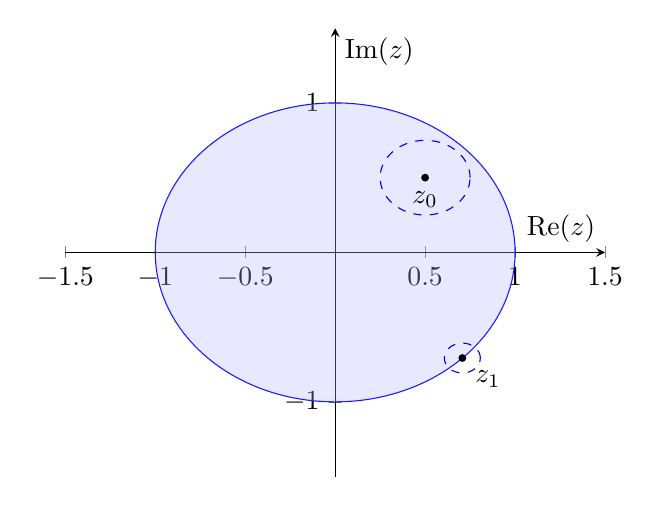
\begin{tikzpicture}
        \begin{axis}[
            axis lines=center,
            ymin=-1.5, ymax=1.5,
            xmin=-1.5, xmax=1.5,
            xlabel=$\operatorname{Re}(z)$, ylabel=$\operatorname{Im}(z)$,
        ]
            \draw[blue] (axis cs: 0, 0) circle (1);
            \fill[blue!30, opacity=0.3] (axis cs: 0, 0) circle (1);
            
            \node[label=-90:$z_0$, circle, fill, inner sep=1pt] at (0.5, 0.5) {};
            \draw[blue, dashed] (axis cs: 0.5, 0.5) circle (0.25);
            
            \node[label=-45:$z_1$, circle, fill, inner sep=1pt] at (0.707, -0.707) {};
            \draw[blue, dashed] (axis cs: 0.707, -0.707) circle (0.1);
        \end{axis}
    \end{tikzpicture}
\end{figure}
\noindent In the figure above, the value $z_0 \in \mathbb{C}$ is not a boundary point of the set since we have an open ball around it that is fully contained in the set. However, $z_1 \in \mathbb{C}$ is a boundary point since any open ball around it will not be fully contained in the set. So, this set is not open since $z_1$ is a boundary point.

As we expect, open discs are open.
\begin{proposition}
Let $z_0 \in \mathbb{C}$ and let $r > 0$. Then, the open disc
\[D = \{z \in \mathbb{C} \mid |z - z_0| < r\}\]
is open.
\end{proposition}
% \begin{proof}
% Let $z \in D$. In that case, $|z - z_0| < r$. Set $\varepsilon = r - |z - z_0| > 0$. So, for $a \in \mathbb{C}$, if $|z - a| < \varepsilon$, then
% \[|z_0 - a| \leq |z_0 - z| + |z - a| < |z_0 - z| + \varepsilon = r.\]
% This implies that $a \in D$. So, $D(a, r)$ is open.
% \end{proof}
\noindent Also, $\mathbb{C}$ is open. This is because for all $z_0, z \in \mathbb{C}$, if $|z - z_0| < 1$, then $z \in \mathbb{C}$.\sidefootnote{The choice of 1 here is arbitrary!} We will normally consider functions with domain an open set.

We now define limits.
\begin{definition}
Let $f: \mathbb{C} \to \mathbb{C}$ be a function, and let $z_0, w \in \mathbb{C}$. We say that the limit
\[\lim_{z \to z_0} f(z) = w\]
if for every $\varepsilon > 0$, there exists a $\delta > 0$ such that for $z \in \mathbb{C}$, if $0 < |z - z_0| < \delta$, then $|f(z) - w| < \varepsilon$.
\end{definition}
\noindent As we saw in real analysis, the sequential characterisation of limits still holds in $\mathbb{C}$.
\begin{proposition}
Let $f: \mathbb{C} \to \mathbb{C}$ be a function, and let $z_0, w \in \mathbb{C}$. Then, the limit 
\[\lim_{z \to z_0} f(z) = w\]
if and only if for every sequence $(z_n)_{n=1}^{\infty}$ in $\mathbb{C} \setminus \{z_0\}$ with $z_n \to z_0$, $f(z_n) \to w$.
\end{proposition}
% % \begin{proof}
% % \hspace*{0pt}
% % \begin{itemize}
% %     \item Assume that the limit $\lim_{z \to z_0} f(z) = w$, and let $(z_n)_{n=1}^{\infty}$ be a sequence in $\mathbb{C} \setminus \{z_0\}$ with $z_n \to z_0$. Let $\varepsilon > 0$. We can find a $\delta > 0$ such that for $z \in \mathbb{C}$, if $|z - z_0| < \delta$, then $|f(z) - w| < \varepsilon$. Moreover, we can find an $N \in \mathbb{Z}_{\geq 0}$ such that for $n \in \mathbb{Z}$, if $n \geq N$, then $|z_n - z| < \delta$. In that case, for $n \in \mathbb{Z}$, if $n \geq N$,
% %     \[|z_n - z| < \delta \implies |f(z_n) - w| < \varepsilon.\]
% %     Therefore, $f(z_n) \to w$.
    
% %     \item Now, assume that the limit $\lim_{z \to z_0} f(z) \neq w$. In that case, there exists an $\varepsilon > 0$ such that for all $\delta > 0$, we can find a $z \in \mathbb{C}$ such that although $0 < |z - z_0| < \delta$, $|f(z) - w| \geq \varepsilon$. So, define the sequence $(z_n)_{n=1}^{\infty}$ in $\mathbb{C} \setminus \{z_0\}$ such that for $n \in \mathbb{Z}_{\geq 1}$, $|z_n - z_0| < \frac{1}{n}$ and $|f(z_n) - w| \geq \varepsilon$. Therefore, we have $z_n \to z_0$ but $f(z_n) \not\to w$.
% % \end{itemize}
% % \end{proof}
% We will now look at some arithmetic results about limits. First, we have the addition property of limits.
% \begin{proposition}
% Let $f, g: \mathbb{C} \to \mathbb{C}$ be functions, and let $c, L_1, L_2 \in \mathbb{C}$ such that the limits
% \[\lim_{z \to c} f(z) = L_1, \qquad \lim_{z \to c} g(z) = L_2.\]
% In that case, the limit
% \[\lim_{z \to c} f(z) + g(z) = L_1 + L_2.\]
% \end{proposition}
% % \begin{proof}
% % Let $\varepsilon > 0$. We can find $\delta_1, \delta_2 > 0$ such that for $z \in \mathbb{C}$, if $0 < |z - c| < \delta_1$, then $|f(z) - L_1| < \frac{\varepsilon}{2}$, and if $0 < |z - c| < \delta_2$, then $|f(z) - L_2| < \frac{\varepsilon}{2}$. So, set $\delta = \min(\delta_1, \delta_2)$. In that case, for $z \in \mathbb{C}$, if $0 < |z - c| < \delta$, then 
% % \[|f(z) + g(z) - L_1 - L_2| \leqslant |f(z) - L_1| + |g(z) - L_2| < \frac{\varepsilon}{2} + \frac{\varepsilon}{2} = \varepsilon.\]
% % So, the limit
% % \[\lim_{z \to c} f(z) + g(z) = L_1 + L_2.\]
% % \end{proof}
% \noindent Next, the scalar multiplication property of limits.
% \begin{proposition}
% Let $f: \mathbb{C} \to \mathbb{C}$ be a function, and let $a, c, L \in \mathbb{C}$ such that the limit
% \[\lim_{z \to c} f(z) = L.\]
% Then, the limit
% \[\lim_{z \to c} af(z) = aL.\]
% \end{proposition}
% % \begin{proof}
% % Let $\varepsilon > 0$.
% % \begin{itemize}
% %     \item If $a = 0$, then we know that $af(z) = 0$ for all $z \in \mathbb{C}$. In that case, set $\delta = 1$. Then, for $z \in \mathbb{C}$ with $0 < |z - c| < \delta$, we find that
% %     \[|af(z) - af(c)| = 0 < \varepsilon.\]
% %     So, the limit
% %     \[\lim_{z \to c} af(z) = aL.\]
    
% %     \item Now, assume that $a \neq 0$. In that case, we can find a $\delta > 0$ such that for $z \in \mathbb{C}$, if $0 < |z - c| < \delta$, then $|f(z) - f(c)| < \frac{\varepsilon}{|a|}$. In that case, for $z \in \mathbb{C}$, if $0 < |z - c|< \delta$, then
% %     \[|af(z) - af(c)| = |a| \cdot |f(z) - f(c)| < |a| \cdot \frac{\varepsilon}{|a|} = \varepsilon.\]
% %     So, the limit
% %     \[\lim_{z \to c} af(z) = aL.\]
% % \end{itemize}
% % \end{proof}
% \noindent Next, the multiplicative property of limits. 
% % We start with a lemma.
% % \begin{lemma}
% % Let $f: \mathbb{C} \to \mathbb{C}$ be a function, and let $c, L \in \mathbb{C}$ such that the limit
% % \[\lim_{z \to c} f(z) = L.\]
% % Then, there exist $M \in \mathbb{R}_{> 0}$ and $\delta > 0$ such that for all $z \in \mathbb{C}$, if $0 < |z - c| < \delta$, then $|f(z)| < M$.
% % \end{lemma}
% % \begin{proof}
% % We know that there exists a $\delta > 0$ such that for $z \in \mathbb{C}$, if $0 < |z - c| < \delta$, then $|f(z) - L| < 1$. So, set $M = 1 + |L|$. In that case, for all $z \in \mathbb{C}$, if $0 < |z - c| < \delta$, then
% % \[|f(z)| < |f(z) - L| + |L| = 1 + |L| = M.\]
% % \end{proof}
% % \noindent Using this result, we prove the multiplicative property of limits.
% \begin{proposition}
% Let $f, g: \mathbb{C} \to \mathbb{C}$ be functions, and let $a, c, L_1, L_2 \in \mathbb{C}$ such that the limits
% \[\lim_{z \to c} f(z) = L_1, \qquad \lim_{z \to c} g(z) = L_2.\]
% In that case, the limit
% \[\lim_{z \to c} f(z) g(z) = L_1 L_2.\]
% \end{proposition}
% % \begin{proof}
% % Let $\varepsilon > 0$. We can find a $\delta_1 > 0$ and $M \in \mathbb{R}_{> 0}$ such that for $z \in \mathbb{C}$, if $0 < |z - c| < \delta_1$, then $|f(z)| < M$. Moreover, we can find a $\delta_2 > 0$ such that for $z \in \mathbb{C}$, if $0 < |z - c| < \delta_2$, then $|g(z) - L_2| < \frac{\varepsilon}{2M}$.
% % \begin{itemize}
% %     \item First, assume that $L_2 = 0$. Set $\delta = \min(\delta_1, \delta_2)$. In that case, for $z \in \mathbb{C}$, if $0 < |z - c| < \delta$, then
% %     \[|f(z) g(z) - L_1 L_2| = |f(z)| \cdot |g(z)| < M \cdot \frac{\varepsilon}{2M} = \frac{\varepsilon}{2} < \varepsilon.\]
% %     This implies that the limit
% %     \[\lim_{z \to c} f(z) - g(z) = L_1 L_2.\]
    
% %     \item Now, assume that $L_2 \neq 0$. In that case, we can find a $\delta_3 > 0$ such that for $z \in \mathbb{C}$, if $0 < |z - c| < \delta_3$, then $|f(z) - L_1| < \frac{\varepsilon}{2|L_2|}$. So, set $\delta = \min(\delta_1, \delta_2, \delta_3)$. In that case, for $z \in \mathbb{C}$, if $0 < |z - c| < \delta$, then
% %     \begin{align*}
% %         |f(z) g(z) - L_1 L_2| &= |f(z) g(z) - f(z) L_2 + f(z) L_2 - L_1 L_2| \\
% %         &\leqslant |f(z) g(z) - f(z) L_2| + |f(z) L_2 - L_1 L_2| \\
% %         &= |f(z)| \cdot |g(z) - L_2| + |L_2| \cdot |f(z) - L_1| \\
% %         &< M \cdot \frac{\varepsilon}{2M} + |L_2| \cdot \frac{\varepsilon}{2|L_2|} = \varepsilon.
% %     \end{align*}
% % \end{itemize}
% % \end{proof}

\subsection{Derivatives in $\mathbb{C}$}
Now, we will look at differentiation in $\mathbb{C}$.
\begin{definition}
Let $f: \mathbb{C} \to \mathbb{C}$ be a function, and let $c \in \mathbb{C}$. Then, we say that $f$ is \emph{differentiable at $c$} if the limit
\[\lim_{z \to c} \frac{f(z) - f(c)}{z - c}\]
exists. If the limit exists, we denote the value by $f'(c)$. We say that $f$ is \emph{differentiable} if $f$ is differentiable at $c$ for all $c \in \mathbb{C}$.
\end{definition}
\noindent Although the difference quotient is the same in $\mathbb{C}$ as in $\mathbb{R}$, there are a lot of functions in $\mathbb{C}$ that we might `expect' to be continuous, but aren't. This is because $\mathbb{R}$ can be thought of as a line, so there are only two directions to approach a point. However, $\mathbb{C}$ is a plane, so there are infinitely many directions we can approach a point from.

We will illustrate the difference with an example. Consider the function $f: \mathbb{C} \to \mathbb{C}$ given by $f(z) = |z|^2 = z \overline{z}$. We can consider the function as a map $g: \mathbb{R}^2 \to \mathbb{R}$ given by $g(x, y) = x^2 + y^2$. This is a differentiable function in $\mathbb{R}^2$ because we can derive it partially with respect to both $x$ and $y$. But, $f$ is only differentiable at $z_0 = 0$. 
\begin{itemize}
    \item If $z_0 = 0$, then
    \[f'(0) = \lim_{z \to 0} \frac{z \overline{z} - 0}{z - 0} = \lim_{z \to 0} \overline{z} = \lim_{z \to 0} x - iy = 0.\]
    Note that if $z = x + iy \to 0$, then we must have $x \to 0$ and $y \to 0$.
    
    \item Now, assume that $z_0 \neq 0$. Define the sequences $x_n = z_0 + \frac{1}{n}$ and $y_n = z_0 + \frac{i}{n}$. We know that $x_n, y_n \to z_0$. Moreover,
    \begin{align*}
        \frac{f(x_n) - f(z_0)}{x_n - z_0} &= \frac{(z_0 + 1/n)(\overline{z_0} + 1/n) - z_0 \overline{z}_0}{1/n} \\
        &= \frac{1/n \cdot z_0 + 1/n \cdot \overline{z}_0 + 1/n^2}{1/n} \\
        &= z_0 + \overline{z}_0 + \frac{1}{n} \to z_0 + \overline{z}_0,
    \end{align*}
    and
    \begin{align*}
        \frac{f(y_n) - f(z_0)}{y_n - z_0} &= \frac{(z_0 + i/n)(\overline{z_0} - i/n) - z_0 \overline{z}_0}{i/n} \\
        &= \frac{-i/n \cdot z_0 + i/n \cdot \overline{z}_0 + 1/n^2}{i/n} \\
        &= -z_0 + \overline{z}_0 - \frac{i}{n} \to -z_0 + \overline{z}_0.
    \end{align*}
    Since $z_0 \neq 0$, we know that $z_0 \neq -z_0$. Therefore, we must find that the limit
    \[f'(z_0) = \lim_{z \to z_0} \frac{f(z) - f(z_0)}{z - z_0}\]
    does not exist by the sequential characterisation of continuity.
\end{itemize}
So, the function $f'(0) = 0$, and is not differentiable at any non-zero point. In fact, we say that it depends on the value of $\theta$, where $z = re^{i \theta}$. That is, the direction we approach in. In this case, we saw two directions- approaching $z_0$ from the real line ($\theta = 0$) and the imaginary line ($\theta = \frac{\pi}{2}$).

Similarly, we can show that the complex conjugation function is not differentiable.
\begin{example}
Let $c \in \mathbb{C}$, and define the function $f: \mathbb{C} \to \mathbb{C}$ by $f(z) = \overline{z}$. Then, $f$ is not differentiable at $c$.
\end{example}
\begin{proof}
Let $z_0 \in \mathbb{C}$. Define the sequences $(x_n)_{n=1}^{\infty}$ and $(y_n)_{n=1}^{\infty}$ in $\mathbb{C}$ by $x_n = z_0 + \frac{1}{n}$ and $y_n = z_0 + \frac{i}{n}$. We know that $x_n, y_n \to z_0$. Moreover,
\[\frac{f(x_n) - f(z_0)}{x_n - z_0} = \frac{\overline{z}_0 + \frac{1}{n} - \overline{z}_0}{1/n} = \frac{1/n}{1/n} = 1 \to 1,\]
and
\[\frac{f(y_n) - f(z_0)}{y_n - z_0} = \frac{\overline{z}_0 - \frac{i}{n} + \overline{z}_0}{i/n} = \frac{-i/n}{i/n} = -1 \to -1.\]
So, the sequential characterisation of continuity tells us that the limit
\[f'(z_0) = \lim_{z \to z_0} \frac{f(z) - f(z_0)}{z - z_0}\]
does not exist.
\end{proof}

% % Nonetheless, there are some basic functions that are differentiable in $\mathbb{C}$, like in $\mathbb{R}$. We start by deriving constant functions.
% % \begin{proposition}
% % Let $a \in \mathbb{C}$, and define the function $f: \mathbb{C} \to \mathbb{C}$ by $f(z) = a$. Then, $f$ is differentiable, with $f'(z) = 0$ for all $z \in \mathbb{C}$.
% % \end{proposition}
% % \begin{proof}[Proof from definition]
% % Let $\varepsilon > 0$, and $c \in \mathbb{C}$. Set $\delta = 1$. In that case, for $z \in \mathbb{C}$, if $0 < |z - c| < \delta$, then
% % \[\left|\frac{f(z) - f(c)}{z - c}\right| = \left|\frac{a - a}{z - c}\right| = 0 < \varepsilon.\]
% % Therefore, $f$ is differentiable at $c$, with $f'(c) = 0$.
% % \end{proof}
% % \begin{proof}[Proof by limits]
% % Let $c \in \mathbb{C}$. We find that
% % \[f'(c) = \lim_{z \to c} \frac{f(z) - f(c)}{z - c} = \lim_{x \to c} \frac{a - a}{z - c} = \lim_{z \to c} 0 = 0.\]
% % \end{proof}
% % \noindent Next, we show that $f(z) = z$ is differentiable.
% % \begin{proposition}
% % Define the function $f: \mathbb{C} \to \mathbb{C}$ by $f(z) = z$. Then, $f$ is differentiable, with $f'(z) = 1$ for all $z \in \mathbb{C}$.
% % \end{proposition}
% % \begin{proof}[Proof by definition]
% % Let $\varepsilon > 0$ and let $c \in \mathbb{C}$. Set $\delta = 1$. In that case, for $z \in \mathbb{C}$, if $0 < |z - c| < \delta$, then
% % \[\left|\frac{f(z) - f(c)}{z - c} - 1\right| = |1 - 1| = 0 < \varepsilon.\]
% % Therefore, $f$ is differentiable at $c$, with $f'(c) = 1$.
% % \end{proof}
% % \begin{proof}[Proof by limits]
% % Let $c \in \mathbb{C}$. We find that
% % \[f'(c) = \lim_{z \to c} \frac{f(z) - f(c)}{z - c} = \lim_{z \to c} \frac{z - c}{z - c} = \lim_{z \to c} 1 = 1.\]
% % \end{proof}
% % \noindent We now prove the power rule.
% % \begin{proposition}
% % Let $n \in \mathbb{Z}_{\geqslant 2}$ and define the function $f: \mathbb{C} \to \mathbb{C}$ by $f(z) = z^n$. Then, $f$ is differentiable, with $f'(z) = nz^{n-1}$ for all $z \in \mathbb{C}$.
% % \end{proposition}
% % \begin{proof}
% % Let $c \in \mathbb{C}$. We find that
% % \begin{align*}
% %     f'(c) &= \lim_{z \to c} \frac{f(z) - f(c)}{z - c} \\
% %     &= \lim_{z \to c} \frac{z^n - c^n}{z - c} \\
% %     &= \lim_{z \to c} \frac{(z - c)(z^{n-1} + cz^{n-2} + \dots + c^{n-1})}{z - c} \\
% %     &= \lim_{z \to c} z^{n-1} + cz^{n-2} + \dots + c^{n-1} = nz^{n-1}.
% % \end{align*}
% % \end{proof}

Using the properties of limits, we can establish arithmetic properties of derivatives. We start with the sum rule.
\begin{proposition}
Let $f, g: \mathbb{C} \to \mathbb{C}$ be functions and let $c \in \mathbb{C}$ such that $f$ and $g$ are differentiable at $c$. Then, $f+g$ is differentiable at $c$, with $(f+g)'(c) = f'(c) + g'(c)$.
\end{proposition}
% % \begin{proof}
% % We find that
% % \begin{align*}
% %     (f+g)'(c) &= \lim_{z \to c} \frac{(f+g)(z) - (f+g)(c)}{z - c} \\
% %     &= \lim_{z \to c} \frac{f(z) + g(z) - f(c) - g(c)}{z - c} \\
% %     &= \lim_{z \to c} \frac{f(z) - f(c)}{z - c} + \frac{g(z) - g(c)}{z - c} \\
% %     &= \lim_{z \to c} \frac{f(z) - f(c)}{z - c} + \lim_{z \to c} \frac{g(z) - g(c)}{z - c} = f'(c) + g'(c).
% % \end{align*}
% % \end{proof}
\noindent Next, we look at the scalar rule.
\begin{proposition}
Let $f: \mathbb{C} \to \mathbb{C}$ be a function and let $a, c \in \mathbb{C}$ such that $f$ is differentiable at $c$. Then, $af$ is differentiable at $c$, with $(af)'(c) = af'(c)$.
\end{proposition}
% % \begin{proof}
% % We find that
% % \begin{align*}
% %     (af)'(c) &= \lim_{z \to c} \frac{(af)(z) - (af)(c)}{z - c} \\
% %     &= \lim_{z \to c} \frac{a(f(z)  f(c))}{z - c} \\
% %     &= a \lim_{z \to c} \frac{f(z) - f(c)}{z - c} = af'(c).
% % \end{align*}
% % \end{proof}
% \noindent We now look at the product rule.
% \begin{proposition}
% Let $f, g: \mathbb{C} \to \mathbb{C}$ be functions and let $c \in \mathbb{C}$ such that $f$ and $g$ are differentiable at $c$. Then, $fg$ is differentiable at $c$, with $(fg)'(c) = f'(c)g(c) + f(c)g'(c)$.
% \end{proposition}
% % \begin{proof}
% % We find that
% % \begin{align*}
% %     (fg)'(c) &= \lim_{z \to c} \frac{(fg)(z) - (fg)(c)}{z - c} \\
% %     &= \lim_{z \to c} \frac{f(z) g(z) - f(z)g(c) + f(z) g(c) - f(c)g(c)}{z - c} \\
% %     &= \lim_{z \to c} f(z) \cdot \frac{g(z) - g(c)}{z - c} + g(c) \cdot \frac{f(z) - f(c)}{z - c} \\
% %     &= \lim_{z \to c} f(z) \cdot \lim_{z \to c} \frac{g(z) - g(c)}{z - c} + \lim_{z \to c} g(c) \cdot \lim_{z \to c} \frac{f(z) - f(c)}{z - c} \\
% %     &= f(c) g'(c) + f'(c) g(c).
% % \end{align*}
% % \end{proof}
\noindent We will now look at the quotient rule. 
% % We start with a lemma.
% % \begin{lemma}
% % Let $f: \mathbb{C} \to \mathbb{C}$ be differentiable at $c \in \mathbb{C}$, with $f(z) \neq 0$. Then, $\frac{1}{f}$ is differentiable at $z$, with
% % \[\left(\frac{1}{f}\right)'(c) = \frac{-f'(c)}{f(c)^2}.\]
% % \end{lemma}
% % \begin{proof}
% % We find that
% % \begin{align*}
% %     \left(\frac{1}{f}\right)'(c) &= \lim_{z \to c} \frac{1/f(z) - 1/f(c)}{z - c} \\
% %     &= \lim_{z \to c} \frac{f(c) - f(z)}{z - c} \frac{1}{f(z) f(c)} \\
% %     &= \lim_{z \to c} \frac{f(c) - f(z)}{z - c} \lim_{z \to c} \frac{1}{f(z) f(c)} \\
% %     &= -f'(c) \cdot \frac{1}{f(c)^2} = \frac{-f'(c)}{f(c)^2}.
% % \end{align*}
% % \end{proof}
% % \noindent Now, we prove the quotient rule.
\begin{proposition}
Let $f, g: \mathbb{C} \to \mathbb{C}$ be functions and let $c \in \mathbb{C}$ such that $g(c) = 0$. In that case, $\frac{f}{g}$ is differentiable at $c$, with
\[\left(\frac{f}{g}\right)'(c) = \frac{f'(c) g(c) - f(c) g'(c)}{g(c)^2}.\]
\end{proposition}
% % \begin{proof}
% % We find that
% % \begin{align*}
% %     \left(\frac{f}{g}\right)'(c) &= \left(f \cdot \frac{1}{g} \right)'(c) \\
% %     &= f'(c) \frac{1}{g}(c) + f(c) \cdot \frac{-g'(c)}{g(c)^2} \\
% %     &= \frac{f'(c) g(c) - f(c) g'(c)}{g(c)^2}.
% % \end{align*}
% % \end{proof}
\noindent Finally, we have the chain rule.
\begin{proposition}
Let $f: \mathbb{C} \to \mathbb{C}$ and $g: \mathbb{C} \to \mathbb{C}$ be functions such that $f$ is differentiable at $c \in \mathbb{C}$ and $g$ is differentiable at $f(c)$. In that case, the composition $g \circ f$ is differentiable at $c$, with
\[(g \circ f)'(c) = g'(f(c)) f'(c).\]
\end{proposition}
% % \begin{proof}
% % Since $f$ is differentiable at $c$, we know that the limit
% % \[\lim_{z \to c} \frac{f(z) - f(c)}{z - c} = f'(c).\]
% % Similarly, since $g$ is differentiable at $c$, we know that the limit
% % \[\lim_{z \to f(c)} \frac{g(z) - g(f(c))}{z - f(c)} = g'(f(c)).\]
% % In that case,
% % \begin{align*}
% %     (g \circ f)'(c) &= \lim_{z \to c} \frac{g(f(z)) - g(f(c))}{z - c} \\
% %     &= \lim_{z \to c} \frac{g(f(z)) - g(f(c))}{f(z) - f(c)} \frac{f(z) - f(c)}{z - c} \\
% %     &= \lim_{z \to c} \frac{g(f(z)) - g(f(c))}{f(z) - f(c)} \cdot \lim_{z \to c} \frac{f(z) - f(c)}{z - c} \\
% %     &= g'(f(c)) f'(c).
% % \end{align*}
% % \end{proof}

We finish by defining holomorphic functions.
\begin{definition}
Let $\Omega$ be an open subset of $\mathbb{C}$. Then, $f$ is \emph{holomorphic} in $\Omega$ if $f$ is differentiable at every $x \in \Omega$.
\end{definition}


\newpage

\section{Power series}
In this section, we will look at power series in $\mathbb{C}$.
\begin{definition}
Let $(a_n)_{n=0}^{\infty}$ be a sequence in $\mathbb{C}$, and let $c, z \in \mathbb{C}$. The power series $\sum a_n(z - c)^n$ is defined by
\[S(z) = \sum_{n=0}^{\infty} a_n (z - c)^n = a_0 + a_1(z - c) + a_2(z - c)^2 + \dots.\]
We refer to the sequence $(a_n)$ as the \emph{coefficient} sequence, $z$ as the \emph{variable}, and $c$ is the \emph{expansion point}. We say that the power series $S(z)$ \emph{converges} at $z_0 \in \mathbb{C}$ if the series $S(z_0)$ converges. Otherwise, we say that it \emph{diverges} at $z_0$. 
\end{definition}
For example, consider the power series
\[S(z) = \sum_{n=0}^{\infty} (z - c)^n,\]
for some $c \in \mathbb{C}$. Then, we saw before that the interval of convergence is the open disc
\[D = \{z \in \mathbb{C} \mid |z - c| < 1\}.\]

We can also consider absolute convergence at a point.
\begin{definition}
Let $S(z)$ be a power series. We say that $S(z)$ \emph{converges absolutely} at $z_0 \in \mathbb{C}$ if the series $S(z_0)$ converges absolutely.
\end{definition}
\noindent Similarly, we can define uniform convergence.
\begin{definition}
Let $S(z)$ be a power series. We say that $S(z)$ \emph{converges uniformly} on some open disc $D \subseteq \mathbb{C}$ if for every $\varepsilon > 0$, there exists an $N \in \mathbb{Z}_{\geq 0}$ such that for $n \in \mathbb{Z}$, if $n \geq N$, then
\[|S_n(z) - S(z)| < \varepsilon\]
for all $z \in D$. We define by $S_n(z)$ the partial sum
\[S_n(z) = \sum_{i=1}^n a_i(z - c)^i.\]
\end{definition}

Now, we define the radius of convergence and its properties.
\begin{theorem}
Let $S(z)$ be a power series. Then, there exists an $R \in [0, \infty)$ such that
\begin{itemize}
    \item $S(z)$ diverges for all $z \in \mathbb{C}$ with $|z - c| > R$;
    \item $S(z)$ converges absolutely and uniformly for all $z \in \mathbb{C}$ with $|z - c| \leq r$, for some $0 \leq r < R$; and
    \item \[R = \sup \{r \geq 0 \mid |a_n| r^n \text{ is a bounded sequence}\}.\]
\end{itemize}
We call $R$ the \emph{radius of convergence}.
\end{theorem}
\noindent It is possible for $S(z)$ to converge for all $z \in \mathbb{C}$, in which case we say that $R = \infty$.

Now, consider the power series
\[S(z) = \sum_{n=0}^\infty z^{2m}, \qquad T(z) = \sum_{n=0}^{\infty} (-1)^n z^{2m}.\]
Since these are geometric series with variables $z_S = z^2$ and $z_T = -z^2$, they both have radius of convergence $R = 1$. Moreover,
\[S(z) = \frac{1}{1 - z^2}, \qquad T(z) = \frac{1}{1 + z^2}.\]
If we consider $\frac{1}{1 - z^2}$ for $z \in \mathbb{R}$, we would have singularities at $z = \pm 1$ and the series would diverge for $|z| \geq 1$. But, $\frac{1}{1 + z^2}$ does not have any singularities for $z \in \mathbb{R}$. Instead, if we look at the complex series, there are singularities at $z = \pm i$.

Like in the real case, we can use the ratio test to characterise the radius of convergence.
\begin{theorem}
Let $(a_n)_{n=0}^{\infty}$ be a sequence in $\mathbb{C}$, and let
\[\lim_{n \to \infty} \frac{|a_{n+1}|}{|a_n|} = L,\]
where $L \in [0, \infty]$. Then, the radius of convergence $R = \frac{1}{L}$.
\end{theorem}
\begin{proof}
We find that
\[\frac{|z_{n+1}(z - c)^{n+1}|}{|a_n (z - c)^n|} = \frac{|a_{n+1}|}{|a_n|} |z - c| \to L|z - c|.\]
So, if $|z - c| < \frac{1}{L}$, then the ratio test tells us that the power series $S(z)$ converges. Moreover, if $|z - c| > \frac{1}{L}$, then the ratio test tells us that the power series $S(z)$ diverges. So, the radius of convergence $R = \frac{1}{L}$.
\end{proof}

We can use the ratio test to show that the derivative has the same radius of convergence. Let
\[S(z) = \sum_{n=0}^{\infty} a_n (z - c)^n\]
have radius of convergence $R$. Then, we have the derivative
\[S'(z) = \sum_{n=1}^{\infty} na_n (z - c)^{n-1} = \sum_{n=0}^{\infty} (n-1) a_{n-1} (z - c)^n.\]
So, the ratio is
\[\left|\frac{a_{n+1}}{a_n}\right| \left(1 + \frac{1}{n}\right) \to \frac{1}{R} \cdot 1 = \frac{1}{R}.\]
Therefore, it has radius of convergence $R$. Similarly, for the antiderivative $F(z) = w + \sum_{n=0}^{\infty} \frac{a_n}{n+1} (z - c)^{n+1}$, we have
\[\lim_{n \to \infty} \left|\frac{a_{n+1}}{a_n}\right| \left(1 - \frac{1}{n+2}\right) \to \frac{1}{R} \cdot 1 = \frac{1}{R}.\]
Therefore, it has radius of convergence $R$.

So, a power series gives us a holomorphic function.
\begin{proposition}
Let 
\[S(z) = \sum_{n=0}^{\infty} a_n (z - c)^n\]
be a power series with radius of convergence $R > 0$. Then, $S: D \to \mathbb{C}$ is holomorphic, where
\[D = \{z \in \mathbb{C} \mid |z - c| < R\},\]
with 
\[S'(z) = \sum_{n=1}^{\infty} a_n n (z - c)^{n+1}.\]
\end{proposition}

\noindent Moreover, every holomorphic function can always be written as a power series. This is not true in the real case. For a power series, it is its own Taylor series, i.e.
\[S(z) = \sum_{n=0}^{\infty} \frac{S^{(n)}(c)}{n!} (z - c)^n.\]
% TODO: Show?
Also, its antiderivative has the same radius of convergence.
\begin{proposition}
Let 
\[S(z) = \sum_{n=0}^{\infty} a_n (z - c)^n\]
be a power series with radius of convergence $R > 0$. Then, $S: D \to \mathbb{C}$ has an antiderivative, where
\[D = \{z \in \mathbb{C} \mid |z - c| < R\},\]
given by
\[F(z) = w + \sum_{n=0}^{\infty} \frac{a_n}{n+1} (z - c)^{n+1},\]
for some $w \in \mathbb{C}$
\end{proposition}

\newpage

\section{Elementary functions}
\subsection{Trigonometric functions}
The exponential function $\exp: \mathbb{C} \to \mathbb{C}$ is given by
\[e^z = \exp (z) = \sum_{n=0}^{\infty} \frac{1}{n!} z^n = 1 + z + \frac{1}{2!} z^2 + \frac{1}{3!} z^3 + \dots,\]
for some $z \in \mathbb{C}$. If we let $(a_n)_{n=1}^{\infty}$ be a sequence in $\mathbb{C}$ defined by $a_n = \frac{1}{n!}$, then
\[\lim_{n \to \infty} \frac{|a_{n+1}|}{|a_n|} = \lim_{n \to \infty} \frac{n!}{(n+1)!} = \lim_{n \to \infty} \frac{1}{n+1} = 0.\]
So, the ratio test tells us that the radius of convergence of the power series $e^x$ $R = \infty$. 

The properties of the real exponential function extend to the complex exponential function. First, the derivative of the exponential function is itself.
\begin{proposition}
Let $z \in \mathbb{C}$. Then, 
\[e'(x) = e(x).\]
\end{proposition}
\begin{proof}
We find that
\begin{align*}
    e'(x) &= \sum_{n=1}^{\infty} \frac{1}{n!} nz^{n-1} \\
    &= \sum_{n=1}^{\infty} \frac{1}{(n-1)!} z^{n-1} \\
    &= \sum_{n=0}^{\infty} \frac{1}{n!} z^n = e(x).
\end{align*}
\end{proof}
\noindent Moreover, the following properties hold.
\begin{proposition}
Let $z, w \in \mathbb{C}$. Then, $e^{z + w} = e^z e^w$ and $e^{-z} = \frac{1}{e^z}$.
\end{proposition}
\begin{proof}
Define the function $f: \mathbb{C} \to \mathbb{C}$ by $f(z) = e^{z + w} e^{-z}$. Then,
\[f'(z) = e^{z + w} e^{-z} + e^{z + w} \cdot -e^{-z} = 0.\]
In that case, $f$ is a constant. Then,
\[f(z) = e^{z + w} e^{-z} = f(0) = e^{0 + w} e^{0} = e^w.\]
So, $e^{z+w} e^{-z} = e^w$ for all $z, w \in \mathbb{C}$. This means that $e^{z+w} = e^z e^w$, and 
\[e^{z+0} e^{-z} = e^0 = 1,\]
and so $e^{-z} = \frac{1}{e^z}$.
\end{proof}

We can further define
\begin{align*}
    \cos (z) &= \frac{e^{iz} + e^{-iz}}{2} = 1 - \frac{z^2}{2!} + \frac{z^4}{4!} - \dots = \sum_{n=0}^{\infty} \frac{(-1)^n}{(2n)!} z^{2n}, \\
    \sin (z) &= \frac{e^{iz} - e^{-iz}}{2i} = z - \frac{z^3}{3!} + \frac{z^5}{5!} - \dots = \sum_{n=0}^{\infty} \frac{(-1)^n}{(2n+1)!} z^{2n+1}.
\end{align*}
% TODO: Show using ratio test
Just using the power series, we will still find that the radii of convergence $R = \infty$. Also, we find that
\begin{align*}
    \cos'(z) &= \sum_{n=1}^{\infty} \frac{(-1)^n}{(2n)!} 2n z^{2n-1} \\
    &= \sum_{n=1}^{\infty} \frac{(-1)^n}{(2n-1)!} z^{2n-1} \\
    &= \sum_{n=0}^{\infty} \frac{-(-1)^n}{(2n+1)!} z^{2n+1} = -\sin(z),
\end{align*}
and
\begin{align*}
    \sin'(z) &= \sum_{n=0}^{\infty} \frac{(-1)^n}{(2n+1)!} (2n+1) \cdot z^{2n} \\
    &= \sum_{n=0}^{\infty} \frac{(-1)^n}{(2n)!} z^{2n} = \cos (z).
\end{align*}
Moreover,
\[e^{iz} = \frac{e^{iz} + e^{-iz}}{2} + \frac{e^{iz} - e^{-iz}}{2} = \cos (z) + i \sin (z).\]
We can also define the following trigonometric functions:
\begin{itemize}
    \item \[\tan (z) = \frac{\sin (z)}{\cos (z)},\]
    \item \[\cosh (z) = \frac{e^z + e^{-z}}{2},\]
    \item \[\sinh (z) = \frac{e^z - e^{-z}}{2}.\]
\end{itemize}

\subsection{Logarithmic function and powers}
In $\mathbb{C}$, the exponential function is not injective, since 
\[e^{z + 2\pi i} = e^z e^{2\pi i} = e^z \cdot 1 = e^z.\]
So, we cannot define the logarithm function as the inverse of $\exp: \mathbb{C} \to \mathbb{C}$. We need to restrict both the domain and the codomain. Similarly, for any $n \in \mathbb{Z}$, the function $z \mapsto z^n$ is not injective, since
\[(z e^{\frac{2\pi i}{n}})^n = z^n.\]
So, we would need to restrict the complex power function to find the inverse. 

To compute the inverse, we can use the inverse function theorem.
\begin{theorem}
Let $\Omega \subseteq \mathbb{C}$ be an open set, and let $f: \Omega \to \mathbb{C}$ be a holomorphic function, and let $z \in \Omega$ such that $f'(z) \neq 0$. Then, there exist open sets $U \subseteq \Omega$ and $V \subseteq \mathbb{C}$ with $z \in U$ and $w = f(z) \in V$, such that $f: U \to V$ is bijective, and $f^{-1}: V \to U$ is holomorphic with
\[\frac{d}{dz} f^{-1}(w) = \frac{1}{f'(z)} = \frac{1}{f'(f^{-1}(w))}.\]
\end{theorem}
\noindent Now, let $z \in \mathbb{C}$. We know that
\[e^z = e^{x + iy} = e^x e^{iy} = e^x (\cos y + i \sin y).\]
For all $x \in \mathbb{R}$, $e^x \neq 0$. Moreover, for all $y \in \mathbb{R}$, we cannot have both $\cos y = 0$ and $\sin y = 0$. Therefore, $e^z \neq 0$. So, the inverse function theorem tells us that there are open sets $U, V$ such that $\exp: U \to V$ is bijective and holomorphic. A possible open set is
\[U = \{z = x + iy \in \mathbb{C} \mid x \in \mathbb{R}, y \in (-\pi, \pi)\}.\]
This choice ensures that for all $u_1, u_2 \in U$, $u_1 - u_2 \neq 2k\pi$, for some $k \in \mathbb{Z}$, and so the function is injective. Moreover,
\[V = \exp(\mathbb{C}) = \mathbb{C} \setminus (-\infty, 0].\]
% We know that $\exp (\mathbb{R}) = (0, \infty)$, and if $\operatorname{Im}(z) \neq 0$, then $e$
% TODO: Prove?
This gives us a bijection $\exp: U \to V$. The inverse function is $\log: V \to U$, and is called the principal branch of the (complex) logarithm.

Now, we will find all the complex logarithms for some $z \in \mathbb{C}$.
\begin{example}
The complex logarithms of $z = -1 + \sqrt{3}$ is given by
\[\log z = \log 2 + \frac{2\pi}{3}i + 2k\pi i,\]
for some $k \in \mathbb{Z}$.
\end{example}
\begin{proof}
We find that
\[|z| = \sqrt{1 + 3} = 2.\]
We have $\arg z = \theta + 2k \pi$ for $k \in \mathbb{Z}$, where $\cos \theta = -1$ and $\sin \theta = \sqrt{3}$. So,
\[\theta = \pi - \tan^{-1} \sqrt{3} = \pi - \frac{\pi}{3} = \frac{2\pi}{3}.\]
Therefore,
\[\log z = \log (|z| e^{i \arg z}) + \log |z| + i \arg z = \log 2 + \frac{2\pi}{3} i + 2k \pi i,\]
for some $k \in \mathbb{Z}$.
\end{proof}

Now, we will define complex powers for a complex number:
\begin{definition}
Let $z, w \in \mathbb{C}$. We define 
\[z^w = e^{w \log z},\]
where $\log z$ are the complex logarithms of $z$.
\end{definition}
\noindent A complex number has many complex logarithms, so we can limit ourselves with the principal branch
\[\log: \mathbb{C} \setminus (-\infty, 0] \to \{z = x + iy \in \mathbb{C} \mid x \in \mathbb{R}, y \in (-\pi, \pi)\}.\]
Then, the function $f: \mathbb{C} \setminus (-\infty, 0] \to \mathbb{C}$ given by $f(z) = z^w$ is a well-defined holomorphic function for all $w \in \mathbb{C}$, and $z^u z^v = z^{u + v}$ for all $u, v \in \mathbb{C}$ and $z \in \mathbb{C} \setminus (-\infty, 0]$.

We will now compute all the values of $z^i$, for some $z \in \mathbb{C}$. By definition, $z^i = e^{i \log z}$. Moreover, we know that
\[\log z = \log |z| + i \arg z.\]
Therefore,
\[z^i = e^{i \log z} = e^{i \log |z|} e^{-\arg z}.\]

\newpage

\section{Cauchy-Riemann equations}
We saw that a vector function $f: \mathbb{R}^2 \to \mathbb{R}$ being differentiable is not equivalent to saying the corresponding function $f: \mathbb{C} \to \mathbb{R}$ is differentiable. In this section, we characterise complex differentiation in terms of vector differentiation. 

Consider a holomorphic function $f: \Omega \to \mathbb{C}$ by
\[f(x + iy) = u(x, y) + iv(x, y).\]
We can see this as a vector function $f: \overline{\Omega} \to \mathbb{R}^2$, where
\[\overline{\Omega} = \{(x, y) \in \mathbb{R}^2 \mid x + iy \in \Omega\} \subseteq \mathbb{R}^2,\]
and $f(x, y) = (u(x, y), v(x, y))$. Since $f$ is differentiable for all $z \in \Omega$, the limit
\[\lim_{h \to 0} \frac{f(z + h) - f(z)}{h}\]
exists, no matter how $h$ approaches $0$. In particular, if we restrict $h = \varepsilon$, for $\varepsilon \in \mathbb{R}$, we find that
\begin{align*}
    \lim_{\varepsilon \to 0} \frac{f(z + \varepsilon) - f(z)}{\varepsilon} &= \lim_{\varepsilon \to 0} \frac{u(x + \varepsilon, y) - u(x, y)}{\varepsilon} + i \lim_{\varepsilon \to 0} \frac{v(x + \varepsilon, y) - v(x, y)}{\varepsilon} \\
    &= \frac{\partial u}{\partial x} + i \frac{\partial v}{\partial x} = \frac{\partial f}{\partial x}.
\end{align*}
Instead, if we restrict $h = i \varepsilon$, for $\varepsilon \in \mathbb{R}$, we find that
\begin{align*}
    \lim_{\varepsilon \to 0} \frac{f(z + i\varepsilon) - f(z)}{i\varepsilon} &= \lim_{\varepsilon \to 0} \frac{u(x, y + \varepsilon) - u(x, y)}{i\varepsilon} + i\lim_{\varepsilon \to 0} \frac{v(x, y + \varepsilon) - v(x, y)}{i \varepsilon} \\
    &= \frac{1}{i} \frac{\partial u}{\partial x} + \frac{i}{i} \frac{\partial v}{\partial y} = -i \frac{\partial f}{\partial y}.
\end{align*}
Therefore,
\[f'(z) = \frac{\partial u}{\partial x} + i \frac{\partial v}{\partial x} = -i \frac{\partial u}{\partial x} + \frac{\partial v}{\partial x}.\]
Equating the real and the imaginary parts, we find that
\[\frac{\partial u}{\partial x} = \frac{\partial v}{\partial y}, \qquad \frac{\partial v}{\partial x} = -\frac{\partial u}{\partial y}.\]
These are the Cauchy-Riemann equations. Geometrically, this means that a differentiable function in $\mathbb{C}$ preserves angles any two lines in the complex plane.

We have shown that if a complex function $f: \Omega \to \mathbb{C}$ is holomorphic, then the vector function $f: \overline{\Omega} \to \mathbb{C}$ must satisfy the Cauchy-Riemann equations. It also turns out that if a vector function $f: \overline{\Omega} \to \mathbb{C}$ satisfies the Cauchy-Riemann equations (and the partial derivatives are continuous), then the complex function $f: \Omega \to \mathbb{C}$ is holomorphic.

\begin{theorem}[Cauchy-Riemann equations]
Let $\Omega \subseteq \mathbb{C}$ be open, and let $w: \Omega \to \mathbb{C}$ be a function, denoted by $w(x + iy) = u(x, y) + iv(x, y)$. Then, 
\begin{itemize}
    \item if $w$ is holomorphic, then $w$ satisfies the Cauchy-Riemann equations, i.e.
    \[\frac{\partial u}{\partial x} = \frac{\partial v}{\partial y}, \qquad \frac{\partial u}{\partial y} = -\frac{\partial v}{\partial x};\]
    \item if $w$ satisfies the Cauchy-Riemann equations and the partial derivatives are continuous, then $w$ is holomorphic.
\end{itemize}
\end{theorem}

We will use the Cauchy-Riemann equations to show that the exponential function is holomorphic in $\mathbb{C}$.
\begin{example}
The function $f: \mathbb{C} \to \mathbb{C}$ given by 
\[f(z) = e^z\]
is holomorphic.
\end{example}
\begin{proof}
For $x + iy \in \mathbb{C}$, we have
\[f(x + iy) = e^{x + iy} = e^x \cos (y) + ie^x \sin (y).\]
Let $u, v: \mathbb{R}^2 \to \mathbb{R}$ be given by $u(x, y) = e^x \cos (y)$ and $v(x, y) = e^x \sin (y)$. Then,
\begin{align*}
    \frac{\partial u}{\partial x} &= e^x \cos (y) & \frac{\partial u}{\partial y} &= -e^x \sin (y) \\
    \frac{\partial v}{\partial x} &= e^x \sin (y) & \frac{\partial v}{\partial y} &= e^x \cos (y).
\end{align*}
So, the Cauchy-Riemann equations are satisfied for all $x + iy \in \mathbb{C}$, and the partial derivatives are continuous. This implies that the function $f$ is holomorphic.
\end{proof}

% \begin{example}
% The function $f: \mathbb{C} \to \mathbb{C}$ given by $f(z) = \overline{z}$ is not differentiable at any $z \in \mathbb{C}$.
% \end{example}
% \begin{proof}
% For $x + iy \in \mathbb{C}$, we have
% \[f(x + iy) = x - iy.\]
% So, let $u, v: \mathbb{R}^2 \to \mathbb{R}$ be given by $u(x, y) = x$ and $v(x, y) = -y$. Then,
% \[\frac{\partial u}{\partial x} = 1 \neq -1 = \frac{\partial v}{\partial y}.\]
% So, the Cauchy-Riemann equations are not satisfied. This implies that $f$ is not differentiable at any $x + iy \in \mathbb{C}$.
% \end{proof}
\newpage

\section{Harmonic functions}
A function $u: \mathbb{R}^2 \to \mathbb{R}$ is harmonic if it satisfies the Laplace equation
\[\frac{\partial^2 u}{\partial x^2} + \frac{\partial^2 u}{\partial y^2} = 0.\]
It turns out that each complex-differentiable function defines two harmonic functions.
\begin{proposition}
Let $f: \mathbb{C} \to \mathbb{C}$ be a holomorphic function. Denote
\[f(x + iy) = u(x, y) + iv(x, y),\]
where $u$ and $v$ have continuous $2$-nd order partial derivatives. Then, $u$ and $v$ are harmonic.
\end{proposition}
\begin{proof}
We find that
\begin{align*}
    \frac{\partial^2 u}{\partial x^2} + \frac{\partial^2 u}{\partial y^2} &= \frac{\partial}{\partial x} \frac{\partial u}{\partial x} + \frac{\partial}{\partial y} \frac{\partial u}{\partial y} \\
    &= \frac{\partial}{\partial x} \frac{\partial u}{\partial y} - \frac{\partial}{\partial y} \frac{\partial u}{\partial x} \\
    &= \frac{\partial^2 u}{\partial x \partial y} - \frac{\partial^2 u}{\partial y \partial x} = 0.
\end{align*}
So, $u$ is harmonic. Similarly, $v$ is harmonic.
\end{proof}

For a complex-differentiable function, we have 2 harmonic functions- one for the real part and one for the complex part. We say that the 2 vector functions are harmonic conjugates.
\begin{definition}
Let $f: \mathbb{C} \to \mathbb{C}$ be a holomorphic function. Denote
\[f(x + iy) = u(x, y) + iv(x, y).\]
We say that $u$ and $v$ are \emph{harmonic conjugates} of each other.
\end{definition}
\noindent We can find the Harmonic conjugate for any harmonic function if the domain is path connected.
\begin{proposition}
Let $\Omega \subseteq \mathbb{C}$ be open and path connected, and let $u: \Omega \to \mathbb{R}$ be harmonic such that $u$ has continuous second order derivatives. Then, $u$ has a harmonic conjugate.
\end{proposition}
\noindent A set $V$ is path connected if for any two values $x_1, x_2 \in V$, there is a path from $x_1$ to $x_2$.
% Illustrate

We will now find the harmonic conjugate for a vector function.
\begin{example}
The function $u: \mathbb{R}^2 \to \mathbb{R}$ given by $u(x, y) = x^3 - 3xy^2$ is harmonic, with a harmonic conjugate
\[v(x, y) = 3x^2y - y^3.\]
\end{example}
\begin{proof}
We find that
\begin{align*}
    \frac{\partial u}{\partial x} &= 3x^2 - 3y^2 & \frac{\partial u}{\partial y} &= -6xy \\
    \frac{\partial^2 u}{\partial x^2} &= 6x & \frac{\partial^2 u}{\partial y^2} &= -6x
\end{align*}
Therefore, the function $u$ is harmonic. Now, let $v: \mathbb{R}^2 \to \mathbb{R}$ be the harmonic conjugate of $u$. We know that
\[3x^2 - 3y^2 = \frac{\partial u}{\partial x} = \frac{\partial v}{\partial y}.\]
So,
\[v = \int 3x^2 - 3y^2 \ dy = 3x^2y - y^3 + f(x),\]
for some $f: \mathbb{R} \to \mathbb{R}$. Moreover, we know that
\[-6xy = \frac{\partial u}{\partial y} = -\frac{\partial v}{\partial x} = -6xy - f'(x).\]
So, $f$ is a constant. Setting $f(x) = 0$, we get the harmonic conjugate
\[v(x, y) = 3x^2y - y^3.\]
\end{proof}
Using this result, we find that there is an analytic function $f: \mathbb{C} \to \mathbb{C}$ given by
\[f(x + iy) = (x^3 - 3xy^2) + i(3x^2y - y^3) = x^3 + 3i x^2y - 3xy^2 -i y^3.\]
In fact, this function is $z \mapsto z^3$.

\end{document}
